\chapter{Fundamentals of Machine Learning and Neural Networks}
\label{ml-fundamentals}

In modern medicine, 
ever increasing amounts of data 
is continuously being generated and collected.
Ranging from structured administrative data 
used primarily for billing purposes
to advanced imaging and high-througput \enquote{omics} analyses,
the array of available data is as diverse as it is plentiful.
Making sense and making use of such massive amounts of data 
necessitates automated methods for data analysis.

% figure: hierarchy of artificial intelligence {{{
\begin{marginfigure}[3em]
    \centering
	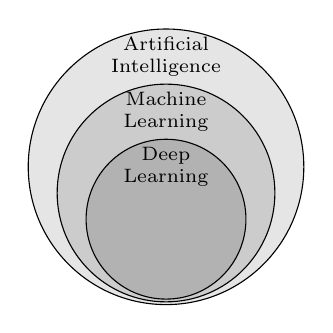
\begin{tikzpicture}[scale=1.75]
        \draw[black, fill=black!10] (0,  0.00) circle (1.00);
        \draw[black, fill=black!20] (0, -0.19) circle (0.79);
        \draw[black, fill=black!30] (0, -0.38) circle (0.58);
        \node[font=\scriptsize, text width=1.8cm, align=center] 
            at (0, 0.8) {Artificial Intelligence};
        \node[font=\scriptsize, text width=1.8cm, align=center] 
            at (0, 0.4) {Machine Learning};
        \node[font=\scriptsize, text width=1.4cm, align=center] 
            at (0, 0.0) {Deep Learning};
	\end{tikzpicture}
    \caption[The hierarchy of artificial intelligence (AI)]{%
        \Ac*{AI} is an umbrella term for computer software 
        that have some sort of \enquote{intelligence} and
        \ac*{ML} is a collection of methods through which 
        that can be achieved. 
        \Ac*{DL}, a specific method in \acs*{ML}, 
        relies on neural networks with many layers
        to analyse complex data.
    }
    \label{fig:artificial-intelligence}
\end{marginfigure}% }}}

\Ac{AI}, and specificically \ac{ML} (\cref{fig:artificial-intelligence}),
seeks to address this need by development of methods and algorithms
that allows computers to \enquote{learn} from data to solve new problems
instead of them being explicitly programmed.
~\autocite{goodfellow2016deep}
The field of \ac{ML} have progressed exponentially
over the past couple of decades, 
and with the advent of generative \ac{AI} models like 
GPT-4~\autocite{openaiGPT42023} and
DALL-E~\autocite{rameshZeroShot2021}
there is a growing public interest in the use of \ac{AI} and \ac{ML}.
In the context of precision medicine,
the promise of \ac{AI} lies in the ability 
to integrate large amounts of data from huge data sets
and register and highlight patterns with clinical importance.
In his review on artificial intelligence in medicine%
\autocite{topolHighperformance2019}, 
Eric Topol expresses his view, that in the not so distant future
\blockquote{%
almost every type of clinician, ranging from specialty doctor to paramedic,
will be using AI technology, and in particular deep learning}.

The underlying principle of \ac{ML} is to formulate a learning problem with a
well-defined objective and a quantifiable measure of performance.
~\autocite{murphyMachine2012}
Subsequently,
a loosely defined computer program is established and fed with data
representing said objective.
Guided by the performance metric, \ac{ML}
algorithms iteratively refine the underlying computer program until the
objective is optimally addressed. 
In his 1997 book \citetitle{mitchellMachine1997},
\citeauthor*{mitchellMachine1997} defines this formally as:
\begin{displayquote}[mitchellMachine1997]
   A computer program is said to learn from experience \(E\)
   with respect to some class of tasks \(T\) and performance measure \(P\),
   if its performance at tasks in \(T\), as measured by \(P\), 
   improves with experience \(E\).
\end{displayquote}
Though this conceptual framework is common to all \ac{ML} models, 
the diversity in \ac{ML} arises from not only the specific \ac{ML} algorithm, 
but also choices regarding objectives, performance metrics, and program attributes. 
These selections introduce the myriad variations and nuances within \ac{ML}, 
which can be broadly categorized into two distinct approaches:
supervised learning
and 
unsupervised learning.
~\autocite{murphyMachine2012}

\section{Supervised Learning}

In supervised learning, models are trained on labeled examples---%
a dataset 
\(\mathfrak{D} = \{(\vec{x}_i, y_i) \mid i \in \{1, \ldots, N\}\} \) 
of size \(N\) that contains both input features \(\vec{x}\)
and corresponding correct output values \(y\)
for all the examples in the dataset. 
Here \( \mathfrak{D} \) is typically refered to as the training set.
~\autocite{murphyMachine2012}
The primary aim in supervised learning 
is to learn a function \(f\) that correctly 
maps input data \(\vec{x}\) to output data \(y\), 
i.e. correctly assigns output labels or values
based on the features present in the input data.
When the output is discrete labels or classes, 
the task is called a classification problem.
Conversely, 
if the output is continuous values,
it is called a regression problem.

Illustrating with a supervised learning task in the domain of classification, 
we can consider a database of coronary angiography images that have been 
manually annotated to indicate the presence or absence of critical stenosis 
in any of the coronary arteries. 
In this scenario, 
the output classes are denoted as 
\(y \in \{\textsf{stenosis}, \textsf{no stenosis}\}\), 
and the objective is to classify the images 
into either of these categories based on their pixel values.
The labeled data is being used to guide and \enquote{supervise}
the model in order for it accurately accomplish this categorisation.

Two other examples of supervised learning tasks is presented in 
\nameref{chap:paper-2} and 
\nameref{chap:paper-3}
within this thesis.
However, these tasks differ from classical supervised learning
in that they involve time-to-event predictions and censored labels.
This subject matter will be elaborated upon in the next chapter:
\nameref{survival-analysis}.

\section{Unsupervised Learning}

In contrast to supervised learning,
unsupervised learning is concerned with finding 
underlying patterns or structures within unlabeled datasets. 
In this paradigm, the algorithm operates without the aid of 
predetermined labels or categories, instead learning from the data itself. 
The aim is to discover intrinsic structure in the dataset, 
which can then be used for tasks such as 
dimensionality reduction, clustering, or anomaly detection.
\sidecite[-8em]{murphyMachine2012}

A canonical example of unsupervised learning is the problem of clustering,
where the objective is to partition a set of objects into subgroups based
on similarity.
\sidecite[-11em]{murphyMachine2012}
Things that are similar should be grouped together and
should be relatively dissimilar to things in other groups.
Defining what constitutes \enquote{similar} 
is therefore a central challenge in clustering;
different measures of similarity often result
in fundamentally different clusterings.%
% card clustering analogy{{{
\sidenote[][-15em]{%
    To illustrate, we can consider a set of playing cards,
    that for convenience is limited to aces, court cards, and tens. 
    One possible clustering groups the cards by suit:
\begin{equation*}
    \begin{array}{@{}c@{}ccccc}
    \{
    &\{ 10\twemoji{heart suit}, 
    &    J\twemoji{heart suit}, 
    &    Q\twemoji{heart suit}, 
    &    K\twemoji{heart suit}, 
    &    A\twemoji{heart suit}
    \}, \\
    &\{ 10\twemoji{spade suit}, 
    &    J\twemoji{spade suit}, 
    &    Q\twemoji{spade suit}, 
    &    K\twemoji{spade suit}, 
    &    A\twemoji{spade suit}
    \}, \\
    &\{ 10\twemoji{diamond suit}, 
    &    J\twemoji{diamond suit}, 
    &    Q\twemoji{diamond suit}, 
    &    K\twemoji{diamond suit}, 
    &    A\twemoji{diamond suit}
    \}, \\
    &\{ 10\twemoji{club suit}, 
    &    J\twemoji{club suit}, 
    &    Q\twemoji{club suit}, 
    &    K\twemoji{club suit}, 
    &    A\twemoji{club suit}
    \}\}
\end{array}
\end{equation*}
Another equally valid clustering groups them by rank:
\begin{equation*}
    \begin{array}{@{}c@{}cccc}
\{ 
   &\{10\twemoji{heart suit},
   & 10\twemoji{spade suit}, 
   & 10\twemoji{diamond suit}, 
   & 10\twemoji{club suit}
\}, \\
   &\{J\twemoji{heart suit}, 
   &  J\twemoji{spade suit}, 
   &  J\twemoji{diamond suit}, 
   &  J\twemoji{club suit}
\}, \\
   &\{Q\twemoji{heart suit}, 
   &  Q\twemoji{spade suit}, 
   &  Q\twemoji{diamond suit}, 
   &  Q\twemoji{club suit}
\}, \\
   &\{K\twemoji{heart suit},
   &  K\twemoji{spade suit},
   &  K\twemoji{diamond suit},
   &  K\twemoji{club suit}
\}, \\
   &\{A\twemoji{heart suit},
   &  A\twemoji{spade suit}, 
   &  A\twemoji{diamond suit}, 
   &  A\twemoji{club suit}
\}\}
\end{array}
\end{equation*}
The choice between these clusterings depends on whether
suits or ranks are considered more important,
which probably depends on the specific card game in question.
This challenge applies to most clustering problems---%
the ideal clustering is usually highly context dependent.
}
% }}}
Clustering lies at the heart of precision medicine:
By identifying distinct subgroups of patients with varying risk profiles, 
clinicians can tailor prevention and treatment strategies more effectively, 
optimizing healthcare outcomes as a result.

In \nameref{chap:paper-1} of this thesis,
we present an example of clustering analysis of patients with 
ischemic heart disease by considering the patterns of comorbidity 
common in subgroups of patients.
The specific methods used in this work is outlined 
in \cref{chap:outline-paper-1}.

\section{Generalization and Overfitting}
\label{overfitting}

% figure: generalization error {{{
\begin{marginfigure}[3em]
    \centering
	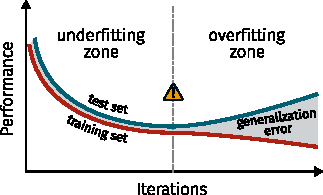
\includegraphics{graphics/overfitting-2}
    \caption[Overfitting as Function of Number of Epochs]{%
        Training a neural network model for many iterations 
        runs the risk of overfitting the model to the training data.
        Although the training error keeps decreasing, 
        it happens at the expense of increased generalization error.
        Inspired by \cite{goodfellow2016deep}.
    }
    \label{fig:generalization-error}
\end{marginfigure}
% }}}

Returning to supervised learning,
it is important to note that achieving good performance on the 
training set is not the sole objective.
For a \ac{ML} model to be of utility, 
it should maintain its accuracy
when applied to unseen data.
This concept is known as \textit{generalization} and
is a central problem in supervised learning---%
especially when dealing with highly flexible models 
such as neural networks.
~\autocite{goodfellow2016deep}
We can keep track of a model's generalization error 
by introducing an additional dataset, 
that is kept separate from the training set. 
This additional set of labeled examples is refered to as the test set
and is exclusively used for evaluation of model performance.
Assuming that the test set is representative%
\sidenote{%{{{
    An underlying assumption is that the two datasets are 
    independent and identically distributed 
    (typically abbreviated as i.i.d.),
    and thus share the same underlying \textit{data-generating process}.
    [\cite{goodfellow2016deep}]
},
% }}}
the performance on the test set can be used as an estimate of 
the generalization error since it represents unseen data.


\Cref{fig:generalization-error} shows a theoretical training history 
of a neural network model where the performance is calculated 
on both a training and a test set after each iteration of the training.
Here it is illustrated that 
the training loss is monotonically decreasing 
with increasing number of iterations.
The validation loss is at first also decreasing,
but if training continues for long enough,
at some point it will start to increase instead.
The divergence between training and test set performance 
indicates overfitting:
instead of learning generalizable patterns representative of the underlying 
data-generating process,
the model starts to learn or even memorise
the noise and idiosyncracies of the data that,
although characteristic in the narrow scope of the training set,
would not be representative of neither biology nor disease etiology.
~\autocite{murphyMachine2012}
As a consequence, the test set performance is considerably worse 
than the training set performance.

% figure: overfitting {{{
\begin{figure}[htb]
	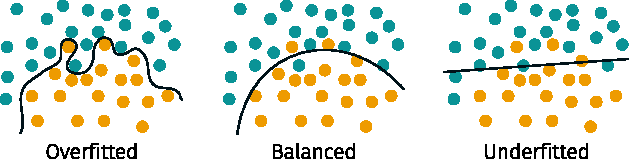
\includegraphics{graphics/overfitting}
    \setfloatalignment{t}
    \caption[What is Overfitting?][-1em]{%
        Illustration of overfitting and underfitting 
        in a simple classification task.
        An overfitted model learns the training data too well,
        and may even remember noise and outliers,
        which makes it perform poorly on unseen data.
        Underfitted models, on the other hand,
        are to simple to capture meaningful patterns in the data.
    }
    \label{fig:overfitting}
    \vspace{-2em}
\end{figure}
% }}}

Overfitting, and its counterpart, underfitting,
are key considerations in training of \ac{ML} models (\cref{fig:overfitting}).
Overfitting happens 
when a model learns the details of the training data too well, 
including the noise, 
which makes it perform poorly on unseen data.
In constrast,
underfitting occurs when the model is too simplistic 
to capture meaningful patterns in the data, 
resulting in poor performance on both the training and test sets.
Both issues highlight the need for balancing the complexity of models,
to ensure that they can effectively generalize to unobserved data.
In the section \nameref{sec:regularization},
I will outline some of the specific methods 
used to balance the complexity 
of neural network models.

\clearpage
\section{Neural Networks}

% figure: neuron{{{
\begin{marginfigure}[3em]
	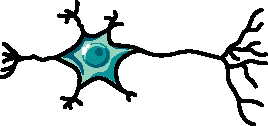
\includegraphics[width=\linewidth]{graphics/neuron}
    \caption[Schematic diagram of a neuron]{%
        Schematic diagram of a neuron.
        A typical neuron has a dendrites, a cell body, and a single axon; 
        the dendrites receive input signals from other neurons,
        and propagates output signals along the axon.
    }
    \label{fig:neuron}
\end{marginfigure}% }}}

In \nameref{chap:paper-2} and \nameref{chap:paper-3}, 
neural network models are utilized to 
develop risk prediction models for ischemic heart disease.
Neural networks is a versatile class of machine learning models
well-suited for handling large and heterogeneous datasets, 
and they currently represent the state-of-the-art in \ac{ML}.
The rest of this chapter will concentrate mainly on neural networks, 
outlining the methodological details and highlight 
relevant practical challenges and considerations 
in their implementation.

Historically, neural networks were designed
using the archicteture of neurons in a human brain as inspiration.
~\autocite{goodfellow2016deep}
The simplest model is that of a perceptron, 
which can be seen as a computational approximation
of a real neuron or nerve cell.
~\autocite{charniakIntroduction2019}
A typical neuron has many dendrites, a cell body, and a single axon 
(\cref{fig:neuron}).
The dendrites carries the input signal to a neuron,
and if the cumulative signal is great enough%
\sidenote[][]{
    This threshold is known as 
    the \textit{threshold potential},
    and is typically between -50 and -55 mV.
}, 
then the neuron will propagate an action potential down the axon%
\autocite{seifterConcepts2005}.
In similar fashion, a perceptron receives may receive many different inputs
and produces a single output (\cref{fig:perceptron}).
In the case of a neuron, the \enquote{all-or-none} principle means
that nerve cells either signals at full strength or not all.
For a perceptron, this principle can be emulated
with the followingly Heaviside step function:
~\autocite{charniakIntroduction2019}

\begin{equation}
    \label{eq:step-function}
    g_{\phi}(\vec{x})  = 
        \begin{cases}
            1 & \text{if } b + \vec{w} \cdot \vec{x} > 0\\
            0 & \text{otherwise}
        \end{cases}
\end{equation}

% figure: perceptron{{{
\begin{marginfigure}%
	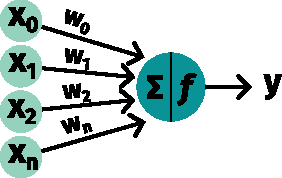
\includegraphics[width=\linewidth]{graphics/perceptron}
	\caption{Schematic diagram of a perceptron}
    \label{fig:perceptron}
\end{marginfigure}% }}}

By combing several of such artificial neurons,
in a multilayer-perceptron or feedforward neural network,
we can create a model that, in theory,
can learn even the most complex of patterns.
~\autocite{bishopNeural1995}
In this design (\cref{fig:nn-structure}),
information travels in one direction, from the input layer
through the hidden layers, and finally to the output layer. 
Each layer in a feedforward neural network is
fully connected to the subsequent layer---%
every neuron in one layer is connected to every neuron in the next.

% figure: neural-network {{{
\begin{figure}[tb]
\tikzstyle{node}        =[thick, circle, draw=color0, minimum size=23, 
                          inner sep=0.5, outer sep=0.6]
\tikzstyle{node in}     =[node, fill=color2]
\tikzstyle{node hidden} =[node, fill=color3]
\tikzstyle{node out}    =[node, fill=color4]
\tikzstyle{connect}     =[thick, color0]
\tikzstyle{label}       =[above=0, align=center, font=\sffamily]
\tikzset{ % node styles,
  node 1/.style={node in},
  node 2/.style={node hidden},
  node 3/.style={node out},
}
\def\nstyle{int(\lay<\Nnodlen?min(2,\lay):3)} % map layer number onto 1, 2, or 3
\centering
\begin{tikzpicture}[x=2.0cm, y=1.0cm]
  \readlist\Nnod{6,4,4,4,5}
  \foreachitem \N \in \Nnod{ % loop over layers
    \def\lay{\Ncnt}  % alias of index of current layer
    \pgfmathsetmacro\prev{int(\Ncnt-1)} % number of previous layer
    \foreach \i [evaluate={\y=\N/2-\i; \x=\lay; \n=\nstyle;}] in {1,...,\N}{
      % nodes
      \node[node \n] (N\lay-\i) at (\x,\y) {};
      % connections
      \ifnum\lay>1
        \foreach \j in {1,...,\Nnod[\prev]}{
          \draw[connect, white, line width=1.2] (N\prev-\j) -- (N\lay-\i);
          \draw[connect] (N\prev-\j) -- (N\lay-\i);
        }
      \fi 
    }
  }
  % labels
  \node[label] at (N1-1.90) { Input };
  \node[label] at (N3-1.90) { Hidden Layers };
  \node[label] at (N5-1.90) { Output };
\end{tikzpicture}
\caption[Schematic of a Feedforward Neural Network]{
    A schematic representation of a feedforward neural network, 
    comprising an input layer, multiple hidden layers, and an output layer. 
    Each circle denotes a neuron, and the connecting lines represent 
    connections between neurons.}
\label{fig:nn-structure}
\end{figure}
% }}}

\subsection{Activation Functions}

In the context of modern neural networks, 
the simplistic step function in \cref{eq:step-function} 
has certain limitations.
In particular, it is non-differentiable at \(x = 0\) and
has a zero derivative elsewhere, 
rendering it incompatible with gradient-based optimization algorithms.  
To address these issues, other activation functions
have been introduced,
with the sigmoid, \ac{tanh}, and \ac{ReLU} being popular choices 
(\cref{fig:act-fn}), but many other variations exists.
~\autocite{cholletDeep2021}

% figure: activation functions {{{
\begin{figure}[htb]
\pgfplotsset{%
    every axis/.append style={%
        tick label style={/pgf/number format/fixed},
        font=\footnotesize,
        ylabel near ticks,
        xlabel near ticks,
        grid=major
    }}
\centering
\begin{tikzpicture}% {{{
    \begin{groupplot}[%
        group style={group size= 2 by 2}, 
        width=0.45\linewidth, height=0.30\linewidth
    ]
    \nextgroupplot[
            title=Heaviside, 
            ylabel= \(g(z)\),
            xmin=-5, xmax=5,
            ymin=-0.30, ymax=1.30
        ]
        \addplot[mark=*, color2, thick, samples at={-5.1, 0},
            mark options={fill=white}]  {0};
        \addplot[mark=*, color2, thick, samples at={0, 5.1},
            mark options={}]  {1};
    %% 
    \nextgroupplot[
            title=Sigmoid, 
            xmin=-5, xmax=5,
            ymin=-0.30, ymax=1.30
        ]
        \addplot[domain=-10:10, color2, thick, samples=100] {1/(1+exp(-x))};
    %% 
    \nextgroupplot[
            title=Tanh, 
            ylabel= \(g(z)\),
            xlabel= \(z\),
            xmin=-5, xmax=5,
            ymin=-1.5, ymax=1.5
        ]
        \addplot[domain=-10:10, color2, thick, samples=100] {tanh(x)};
    \nextgroupplot[
            title=ReLU, 
            xlabel= \(z\),
            xmin=-5, xmax=5,
            ymin=-0.5, ymax=5
        ]
        \addplot[domain=-10:0, color2, thick] {0};
        \addplot[domain=0:10,  color2, thick] {x};
        
    \end{groupplot}
\end{tikzpicture}% }}}
\caption[Well-known Activation Functions]{%
    Plots of well-known activation functions used in neural networks. 
    From top left to bottom right: 
    The Heaviside step function, 
    the sigmoid (or logistic) function,
    the \acf{tanh}, and the \acf{ReLU}.
    Each function is plotted against its input value \(z\) 
    to show its respective output \(g(z)\).}
\label{fig:act-fn}
\end{figure}% }}}

\subsection{Neural Network Architectures}

In addition to feed forward neural networks, 
ongoing research have developed other neural network architectures 
tailored to particular types of data. 
For example, convolutional neural networks were designed 
for processing image data
~\autocite{lecunHandwritten1989}
and have revolutionized the field of
computer vision.
~\autocite{prince2023understanding}
Similarly, recurrent neural networks,
such as the long short-term memory nework,
can model sequential data
and have had great impact for both time series analysis 
and natural language processing.
~\autocite{hochreiterLong1997}
Another innovation, 
is the introduction of skip or residual connections 
in architectures such as residual networks (ResNet),
which have enabled the training of exceptionally deep networks.
~\autocite{heDeep2015}

\clearpage

\section{Practical Implementation of Neural Networks}

In developing neural network models for \ac{ML} objectives,
several methodological considerations and decisions 
have to be made.
It is not feasible to exhaustively cover
every nuance within the scope of this thesis, 
instead the book \citetitle{goodfellow2016deep} 
serves as a comprehensive reference.%
~\sidecite[-3em]{goodfellow2016deep}
As a guide, 
the following list provides a high-level overview of the typical workflow:%
\sidenote[][-4em]{%{{{
    The list draws inspiration from chapter 19.9 in 
    \cite{russellArtificial2009} and chapter 4 in
    \cite{cholletDeep2021}.
}% }}}

\begin{fullwidth}
%\setcounter{unbalance}{3}
\begin{multicols}{2}
\raggedcolumns
\begin{enumerate}
    \item \label{itm:problem}
        \textit{Problem Definition:} 
        Clearly describe the problem, 
        and in the process identify if the objective belongs to 
        classification, regression, or a third category.
        Attached to the objective should be a measure of performance, 
        which in the neural network literature typically is known as 
        loss function, which is used to direct training.

    \item \textit{Preparing the Data}:

        \begin{enumerate}
        \item \label{itm:data-collection}
            \textit{Data Collection:} 
            Gather and organize data for both training and testing the model.
            Importantly, data should be of reasonable quality,
            pertinent to the problem at hand, and of sufficient quantity.
            If not, it can be a good idea to adjust \cref{itm:problem} 
            to better reflect the available data.

        \item \label{itm:data-preprocessing}
            \textit{Data Preprocessing:} 
            Prepare the data for model training, 
            which may include cleaning, normalization, and transformation tasks.
            The classical saying \enquote{garbage in, garbage out}
            is worth repeating here.
            Any data-informed tasks (e.g. normalization) should exclusively
            be setup using the training set to avoid leakage of data.
            \unskip\footnotemark
        \end{enumerate}

    \item \label{itm:model-specification}
        \textit{Network Structure:} 
        Choose the architecture of the neural network, 
        defining elements such as the number of layers, 
        number of neurons within each layer, 
        and activation functions.
        Certain architectures have shown to be useful for specific 
        types of data, e.g. convolutional neural networks are
        typically the architecture of choice for computer vision tasks.%
        \unskip\footnotemark
        
    \columnbreak
    \item \label{itm:training-specification}
        \textit{Configuring Model Training:}
        \begin{enumerate}%
        \item \label{itm:optimizer}
            \textit{Optimization Algorithm:} 
            Choose and configure an optimization algorithm.
            \Ac{SGD} and variants thereof 
            are the most common algorithms for neural networks,
            \unskip\footnotemark
            and all have different 
            parameters that needs to be defined and possibly tuned 
            (see \cref{itm:hyperparameter}), 
            such as e.g. the learning rate.

        \item \label{itm:regularization}
            \textit{Regularization:} 
            To mitigate overfitting and ensure better generalization,
            consider using regularization techniques such as 
            L1/L2-regularization or Dropout.
            \unskip\footnotemark
        \end{enumerate}

    \item \label{itm:hyperparameter}
        \textit{Hyperparameter Tuning:} 
        Tweak and adjust the relevant hyperparameters specified
        in any of the previous steps,
        including learning rate (from \cref{itm:optimizer})
        and specific details of the neural network architecture 
        (\cref{itm:model-specification})
        to find the best configuration.
        This typically involves training many different intermediate
        versions of the model and evaluating their performance
        using a validation set.

    \item \label{itm:training}
        \textit{Model Training:} 
        Train the final version of the model 
        using the designated training set.

    \item \label{itm:evaluation}
        \textit{Model Evaluation:} 
        Assess the trained model using the test set, 
        calculating metrics like accuracy, precision, and recall 
        to gauge its effectiveness.
        Model explainability techniques can here 
        be helpful in aiding the interpretation of the model.
\end{enumerate}
\end{multicols}
\end{fullwidth}

\footnotetext{\cite{cholletDeep2021}}
\footcitetext{lecunHandwritten1989}
\footcitetext{cholletDeep2021}
\footcitetext{goodfellow2016deep}

While presented as sequential steps, 
the items in the list are almost all interrelated 
and can and should affect one another. 
As an example, 
it especially evident that
\cref{itm:data-collection} 
drastically influences the range of possibilities in 
\cref{itm:problem}.
In the remaining sections of this chapter, 
I will be highlighting select concepts integral to  
building neural network models which have specific
relevance to the papers included in the thesis.

\section{Model Selection}
\label{sec:model-selection}

We can estimate the generalization error of a model
by evaluating it on a test set.
If we are only creating a single model,
then this approach suffices. 
However, we might want to compare many different models,
or slightly tweak an already existing model,
such that we can select the best performing version.
This is particularly relevant in the context of hyperparameter optimization,
a topic that I will return to later in this chapter.
If we select the final model based on the test set alone,
we might inadvertently have biased the process,
and could, in a sense, have overfitted to the test data.
~\autocite{murphyMachine2012}
To avoid this, we need to completely hide away the test data
until we are done with training, experimenting, 
and model selection.
To enable this, a common solution is to introduce a third dataset by splitting 
the training data into two sets of data: a training set and a validation set.
The three sets of data used in the development process is then: 
%
\begin{itemize}
    \item a training set to train or develop candidate models
    \item a validation set to evaluate and select the best model
    \item a test set for the final evaluation of model performance
\end{itemize}

\section{Regularization}
\label{sec:regularization}

Regularization is a collection of strategies used to avoid
overfitting by penalizing the complexity of \ac{ML} models.
Two classical examples are L2 and L1 regularization
that adds an regularization term \(\omega\),
on the model parameters \(\phi\),
to the loss function \(\mathcal{L}\).
~\autocite{goodfellow2016deep}

\vspace{1.5em}
\begin{equation}
    \widetilde{\mathcal{L}} (\vec{\phi} , \mathsf{X}, \vec{y}) =
    \mathcal{L} (\vec{\phi} , \mathsf{X}, \vec{y}) +
    \eqnmarkbox[color2]{node1}{ \omega (\vec{\phi})}
\end{equation}
\annotate[yshift=.5em]{left}{node1}{regularization term}

In the case of L1 regularization, 
the regularization term consists of 
the sum of the absolute values of the model parameters, 
also known as the L1 norm. 
For L2 regularization, 
the term comprises the sum of the squares of the model parameters, 
otherwise known as the squared L2 norm.
~\autocite{murphyMachine2012}
%
\begin{alignat}{3}
    &L1: \quad \omega (\vec{\phi}) 
        &&= \lambda||\vec{\phi}||_1 
        &&= \lambda\sum_{i}|\phi_i|  \\
    &L2: \quad \omega (\vec{\phi}) 
        &&= \lambda||\vec{\phi}||_2^2 
        &&= \lambda\sum_{i} \phi_i^2
\end{alignat}

The regularization strength is controlled by a hyperparameter, \(\lambda\);
a value close to zero imposes minimal regularization, 
while larger values increases the amount.
In the context of neural networks, 
another commonly used regularization method is \textit{dropout}.
~\autocite{srivastava2014dropout}
This method simply involves randomly dropping some of the output features
of the hidden layers during each iteration of the training.
This process in a sense creates a different architecture at every step,
discouraging the model from becoming overly dependent on any single feature 
and thereby enhances generalization. 
~\autocite{charniakIntroduction2019}
Empirically, dropout have been found to give significant improvements across
many different architectures 
~\autocite{srivastava2014dropout}
and is a consequence broadly utilized.
~\autocite{charniakIntroduction2019}
The droput rate, which controls the probability \(p\) of dropping out each
individual unit, is a hyperparameter that needs to be specified.

\section{Hyperparameter Optimization}

Neural networks, as well as most other \ac{ML} models,
have parameters and settings that are not adjusted 
during training and therefore needs to pre-specified.
~\autocite{goodfellow2016deep}
These parameters are known as hyperparameters, 
and common examples include aspects such as 
learning rate,
number of layers in the neural network,
number of nodes in each layer,
Other specific examples have also been described previously in this chapter.

Although it is possible to assign default values to hyperparameters 
based on prior experience and personal preference, 
it is imperative to acknowledge their possible impact on model performance.
Consequently, it is common to explore different setting and combinations
of hyperparameters in the model building process.
~\autocite{goodfellow2016deep}
In the field of machine learning, this process is known as \ac{HPO}.

If the number of hyperparameters are sufficiently small,
a commonly employed strategy for \ac{HPO} 
is creating a range of possible candidate values 
for each hyperparameter and 
simply testing the entire space of 
possible combinations in what is known as a \emph{grid search}.
The disadvantage is, however, that the search space quickly 
explodes in size and this strategy may therefore not be feasible.
An alternative strategy, 
which have been emprirically and theoretically shown to outperform
grid search, and therefore typically should be prefered,  
is \emph{random search}.
~\autocite{bergstraRandom2012}
In random search, the hyperparameters values are neither binned nor
discretized and are instead sampled from a uniform distribution.
~\autocite{bergstraRandom2012}
State-of-the-art \ac{HPO} approaches includes Bayesian optimization 
models, multi-fidelity optimization, and metaheuristics algorithms.
~\autocite{yangHyperparameter2020}
Many of these algorithms are implemented in the 
open-source Python package \textit{Optuna},
a very popular software framework for \ac{HPO} in Python.
~\autocite{akibaOptuna2019}

\section{Model Explainability}

As described above, the overall goal of \ac{ML} 
is to make accurate predictions on unseen data,
and the \enquote{how} and \enquote{why} of such predictions is,
in the general \ac{ML} paradigm, 
explicitly of little concern.
Consequently, it is accepted that complex neural networks
with deep architectures and many thousands of parameters 
are \enquote{black box} models that can not 
be easily described nor understood.
~\autocite{russellArtificial2009}
For many applications, 
this lack of transparency can be accepted,
but for other applications where trust is paramount, 
including precision medicine,
ongoing efforts seeks to adress this inherent limitation.
~\autocite{vanderveldenExplainable2022}

\subsection{Interpretability and Explanability}

In the discussion of \ac{XAI}, there is 
a meaningful distinction to be made between 
interpretability and explainability:
A model is said to be interpretable if we can 
relatively easily understand the model through inspection
of the model itself.
~\autocite{russellArtificial2009}
An explainable model, on the other hand, is a simplified 
external process that provides an interpretable approximation
of the complex non-interpretable model.
~\autocite{lundbergUnified2017}
For neural networks,
model explainability techniques are generally 
the only available option.

\subsection{What is SHAP Analysis?} 

A popular method for explainability analysis of neural network models
is \ac{SHAP}, first published by
\citeauthor{lundbergUnified2017} in \citeyear{lundbergUnified2017}
~\autocite{lundbergUnified2017}.
SHAP is a model-agnostic method grounded in co-operative game theory
that provides a unified measure of feature importance for \ac{ML} models.
It is based on the concept of Shapley values,  
an approach for fairly distributing payoffs in a coalitional game
based on the individual contributions of the players.
~\autocite{shapley1953value}
In this framework, 
the \enquote{payoff} is the model output, 
and the \enquote{players} are the features.
For a specific realisation \(\check{\mathbf{x}}\) 
of the feature vector \(\mathbf{x}\),
we then decompose the model output \(f(\check{\mathbf{x}})\)
into the individual feature contributions \(\check{v}_{j}\).
~\autocite{aasExplaining2020}
\begin{equation}
    \label{eq:explain}
    f(\check{\mathbf{x}}) \approx v_0 + \sum_{j=1}^{M} \check{v}_{j}
\end{equation}
where \(v_0\) is a shared baseline and 
\(\check{v}_{i}\) is the marginal contribrution for the \(j\)th 
feature in \( \check{\mathbf{x}}\).
The shared baseline is typically \(\EX[f(\mathbf{x})]\), 
either the average or median prediction from the training set.
~\autocite{aasExplaining2020}
With this formulation, the Shapley values represent the difference between
the prediction \(f(\check{\mathbf{x}})\) and the reference prediction,
and from \cref{eq:explain} it follows that these are additive.
~\autocite{aasExplaining2020}
This enables visualizations such as \cref{fig:shap-local}.

% figure: shap explanations{{{
\begin{figure}[hbt]
    \begin{tikzpicture}[%
        x=\linewidth/100, 
        y=2.7cm/100, 
        font=\footnotesize
    ]
    \tikzstyle{shap}=[line width=11, -{Triangle Cap[]}]

    \node (0) at (0,   50)  {};
    \node (1) at (100, 50)  {};
    \draw (0) -- (1);

    \node (efz0) at (15, 100) { \(\EX [f(\mathbf{x})]\)};
    \node (efz1) at (30,  85) { \(\EX [f(\mathbf{x}) \mid x_1         = \check{x}_{1}]\)};
    \node (efz2) at (45, 100) { \(\EX [f(\mathbf{x}) \mid x_{1,2}     = \check{x}_{1,2}]\)};
    \node (efz3) at (85, 100) { \(\EX [f(\mathbf{x}) \mid x_{1,2,3}   = \check{x}_{1,2,3}]\)};
    \node (efz4) at (69,  85) { \(\EX [f(\mathbf{x}) \mid x_{1,2,3,4} = \check{x}_{1,2,3,4}]\)};
    \node[fill=color4!50!white, draw=color5] 
          (fx)   at (50,  70) { \(f(\mathbf{\check{x}})\)};

    \draw[->, color2, shap] (efz0 |- 50, 40) -- node[white] {\(\check{v}_{1}\)} (efz1 |- 50, 40);
    \draw[->, color2, shap] (efz1 |- 50, 25) -- node[white] {\(\check{v}_{2}\)} (efz2 |- 50, 25);
    \draw[->, color2, shap] (efz2 |- 50, 10) -- node[white] {\(\check{v}_{3}\)} (efz3 |- 50, 10);
    \draw[->, color6, shap] (efz3 |- 50, 25) -- node[white] {\(\check{v}_{4}\)} (efz4 |- 50, 25);
    \draw[->, color6, shap] (efz4 |- 50, 40) -- node[white] {\(\check{v}_{5}\)} (fx   |- 50, 40);

    \foreach \n in {efz0, efz1, efz2, efz3, efz4, fx}
        \draw[->] (\n) -- ($(0)!(\n)!(1)+(0,1)$);

    \end{tikzpicture}
    \caption[Shapley Additive Explanations]{%
       \Acf{SHAP} values represents the difference between the specific model
       output \(f(\check{\mathbf{x}})\) and a baseline prediction
       \(\EX [\mathbf{x}]\). 
       The SHAP values \(v_i\) are additive and by adding them to the 
       baseline prediction, we effetively condition the expected
       model prediction on that feature.
    }
    \label{fig:shap-local}
    \vspace{-2em}
\end{figure}% }}}

It is beyond the scope of this thesis to detail 
how Shapley values are computed in the \ac{SHAP} framework.
However, it is important to note that their exact calculation 
is NP-complete and therefore computationally intractable.
~\autocite{dengComplexity1994}
Instead, the \ac{SHAP} method have pioneered different 
clever approximations that can be computed in reasonable time.
~\autocite{lundbergUnified2017}

